\documentclass[border=10pt]{standalone}
\usepackage{pgfplots}
\pgfplotsset{compat=1.18}
\begin{document}
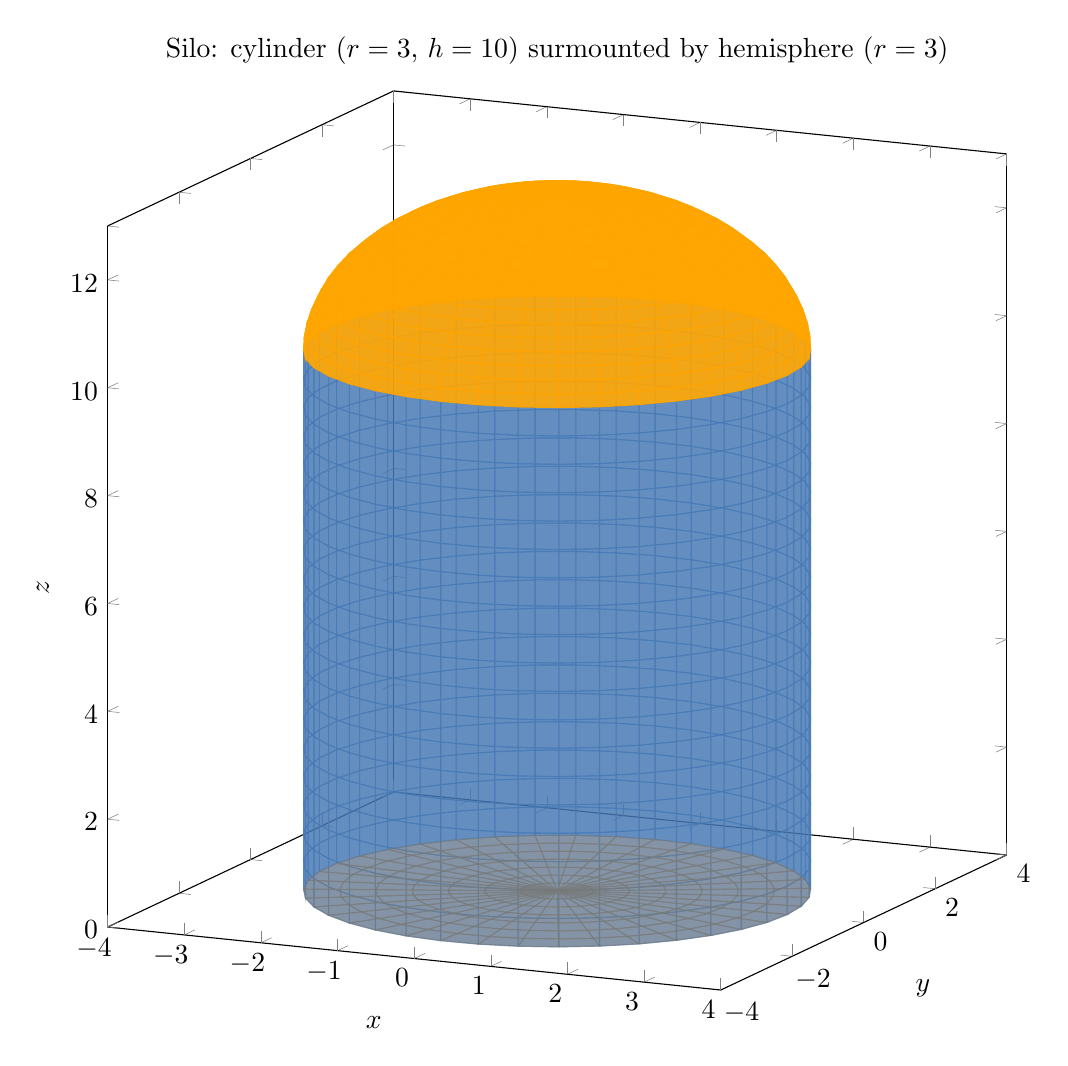
\begin{tikzpicture}
\begin{axis}[
    view={25}{12},
    width=13cm, height=13cm,
    xlabel={$x$}, ylabel={$y$}, zlabel={$z$},
    xmin=-4, xmax=4, ymin=-4, ymax=4, zmin=0, zmax=13,
    title={Silo: cylinder ($r=3$, $h=10$) surmounted by hemisphere ($r=3$)},
]
% Cylinder side surface
\addplot3[surf, shader=flat, z buffer=sort, opacity=0.6,
    colormap={cyl}{rgb255=(70,120,180) rgb255=(70,120,180)},
    domain=0:360, y domain=0:10, samples=40, samples y=20]
    ({3*cos(x)}, {3*sin(x)}, {y});
% Hemisphere dome
\addplot3[surf, shader=flat, z buffer=sort, opacity=0.9,
    colormap={dome}{rgb255=(255,165,0) rgb255=(255,165,0)},
    domain=0:360, y domain=0:90, samples=40, samples y=20]
    ({3*sin(y)*cos(x)}, {3*sin(y)*sin(x)}, {10 + 3*cos(y)});
% Bottom disk
\addplot3[surf, shader=flat, z buffer=sort, opacity=0.5,
    colormap={bot}{rgb255=(120,120,120) rgb255=(120,120,120)},
    domain=0:360, y domain=0:3, samples=40, samples y=8]
    ({y*cos(x)}, {y*sin(x)}, {0});
\end{axis}
\end{tikzpicture}
\end{document}
